%%%%%%%%%%%%%%%%%%%%%%%%%%%%%%%%%%%%%%%%%%%%%%%%%%%%%%%%%%%%%%%%%%%%%%
% Overleaf (WriteLaTeX) Example: Molecular Chemistry Presentation
%
% Source: http://www.overleaf.com
%
% In these slides we show how Overleaf can be used with standard 
% chemistry packages to easily create professional presentations.
% 
% Feel free to distribute this example, but please keep the referral
% to overleaf.com
% 
%%%%%%%%%%%%%%%%%%%%%%%%%%%%%%%%%%%%%%%%%%%%%%%%%%%%%%%%%%%%%%%%%%%%%%

\documentclass{beamer}

\mode<presentation>
{
  \usetheme{Madrid}       % or try default, Darmstadt, Warsaw, ...
  \usecolortheme{default} % or try albatross, beaver, crane, ...
  \usefonttheme{default}    % or try default, structurebold, ...
  \setbeamertemplate{navigation symbols}{}
  \setbeamertemplate{caption}[numbered]
} 

\usepackage[english]{babel}
\usepackage[utf8x]{inputenc}
\usepackage{chemfig}
\usepackage[version=3]{mhchem}

\usepackage{hyperref}
  \hypersetup{colorlinks=true}
  \hypersetup{urlcolor=blue}
  \hypersetup{linkcolor = .}
\usepackage{xcolor}
\usepackage{siunitx}
  \sisetup{separate-uncertainty = true}
\usepackage{physics}
\usepackage[font=small,labelfont=bf]{caption}
\usepackage{subcaption}
\usepackage[en-GB]{datetime2}
\usepackage{feynmp}
\DeclareGraphicsRule{*}{mps}{*}{}

\usepackage{scalerel}
\newcommand{\mylbrace}[2]{\vspace{#2pt}\hspace{6pt}\scaleleftright[\dimexpr5pt+#1\dimexpr0.06pt]{\lbrace}{\rule[\dimexpr2pt-#1\dimexpr0.5pt]{-4pt}{#1pt}}{.}}
\newcommand{\myrbrace}[2]{\vspace{#2pt}\scaleleftright[\dimexpr5pt+#1\dimexpr0.06pt]{.}{\rule[\dimexpr2pt-#1\dimexpr0.5pt]{-4pt}{#1pt}}{\rbrace}\hspace{6pt}}

% Here's where the presentation starts, with the info for the title slide
\title[BESIII Oxford]{BESIII Oxford Group Meeting}
\author{Martin Tat}
\institute{Oxford LHCb}
\date{15th April 2021}

\titlegraphic{
\includegraphics[width = 5cm, height = 3.8cm]{lhcb.jpg}\hspace{1cm}~%
              
\includegraphics[width = 5cm, height = 3.8cm]{bes3.jpg}}

\begin{document}

\begin{frame}
  \titlepage
\end{frame}

% These three lines create an automatically generated table of contents.
%\begin{frame}{Outline}
%  \tableofcontents
%\end{frame}

\section{Intorduction}
\begin{frame}{Introduction}
  \begin{itemize}
    \setlength\itemsep{2em}
    \item{$D\to K^+K^-\pi^+\pi^-$ analysis}
    \item{Previously: Fit to $\Delta E$ and $m_\text{BC}$ to get $KK\pi\pi$ ST yield}
    \begin{itemize}
      \item{Issue: Strange $\Delta E$ shape}
    \end{itemize}
    \item{Current progress:}
    \begin{itemize}
      \item{Found possible explanation for $\Delta E$ shape}
      \item{Looked at $K_SKK$ background, found asymmetric veto range}
    \end{itemize}
  \end{itemize}
\end{frame}

\begin{frame}{MC samples}
  \centering
  \begin{tabular}{ccc}
    MC sample & Events ($10^6$) & Luminosity scale ($2010$/$2011$) \\
    \hline
    $D^0\bar{D^0}$     & $74$   & $21.8$/$21.8$ \\
    $D^+D^-$           & $29$   & $10.9$/$10.8$ \\
    $q\bar{q}$         & $122$  & $7.8$/$7.3$   \\
    $\psi(2S)\gamma$   & $34$   & $10.8$/$10.1$ \\
    $J/\psi\gamma$     & $22$   & $10.8$/$10.1$ \\
    $\tau\tau$         & $60$   & $10.8$/$10.1$ \\
    non-$D\bar{D}$     & $10$   & $10.8$/$10.1$ \\ \\ \\
  \end{tabular}
  \begin{itemize}
    \item{Did not run over $ee$ and $\mu\mu$ MC}
  \end{itemize}
\end{frame}

\section{$\Delta E$ fit in data vs MC}
\begin{frame}{Previous $\Delta E$ fit in data vs MC}
  \begin{figure}
    \centering
    \begin{subfigure}{0.5\textwidth}
      \centering
      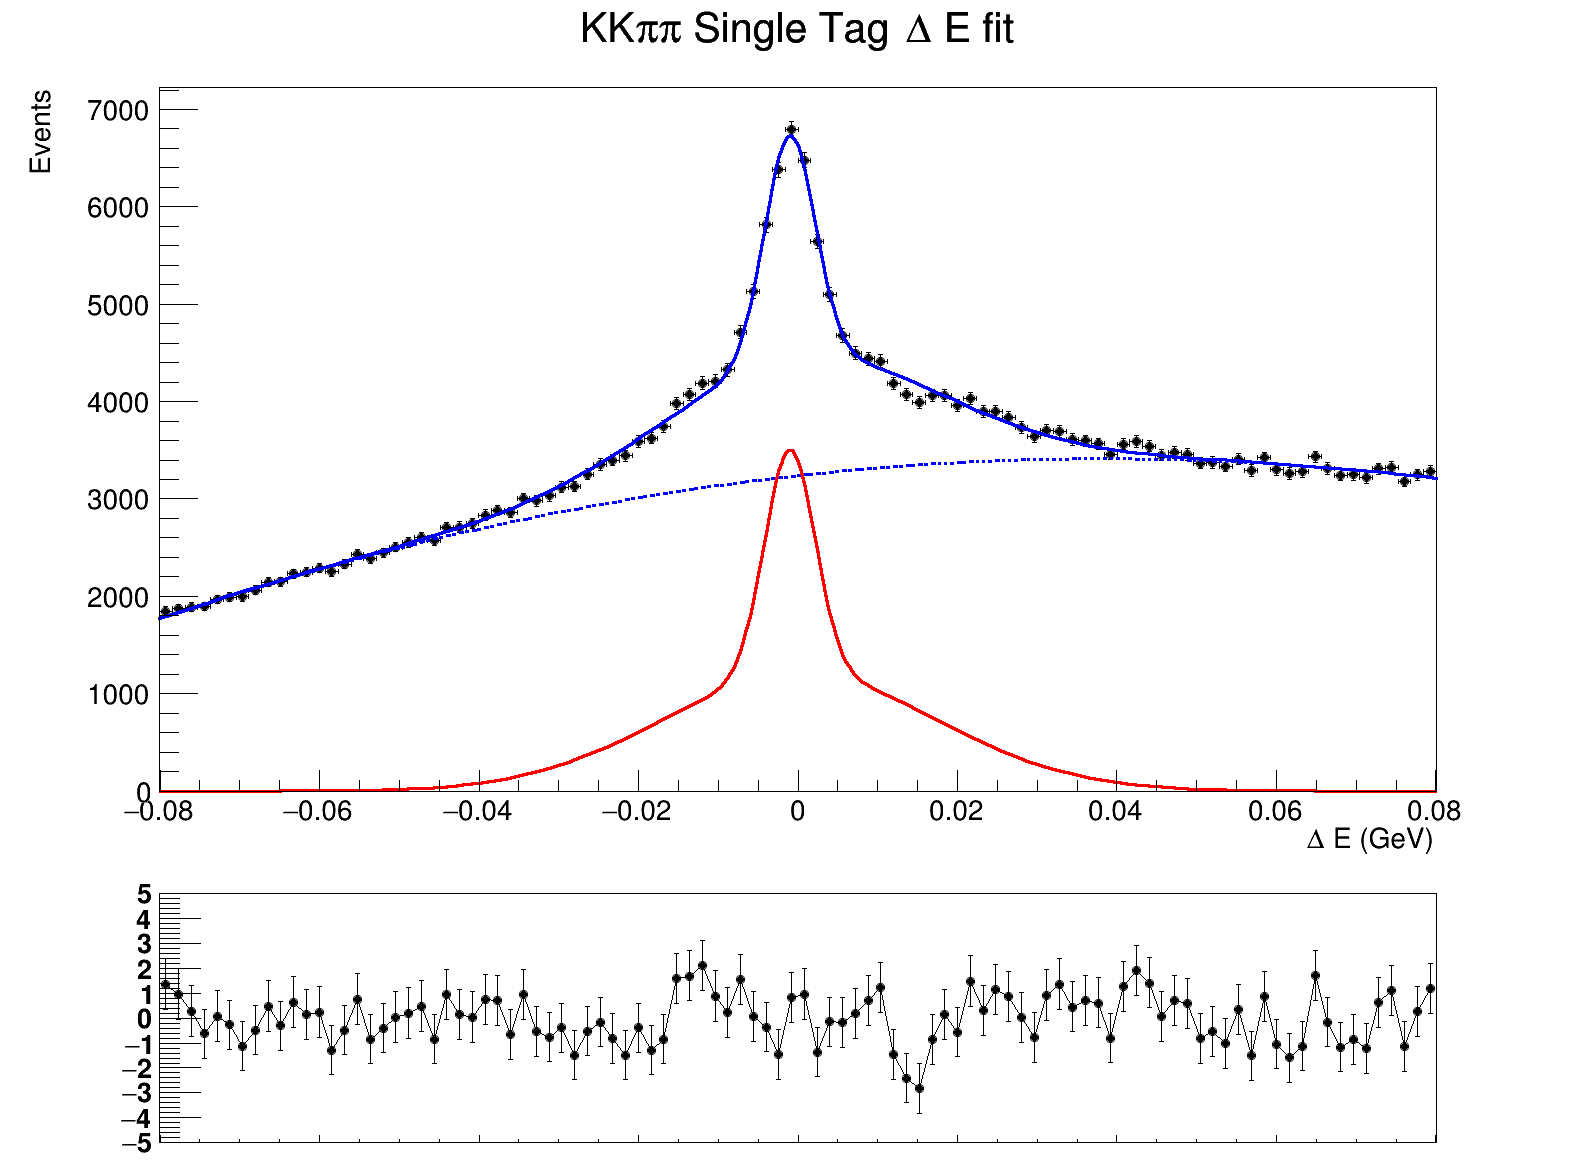
\includegraphics[width=\textwidth]{KKpipiSingleTagDeltaEPlotDataOld.png}
      \caption{$\Delta E$, data}
    \end{subfigure}%
    \begin{subfigure}{0.5\textwidth}
      \centering
      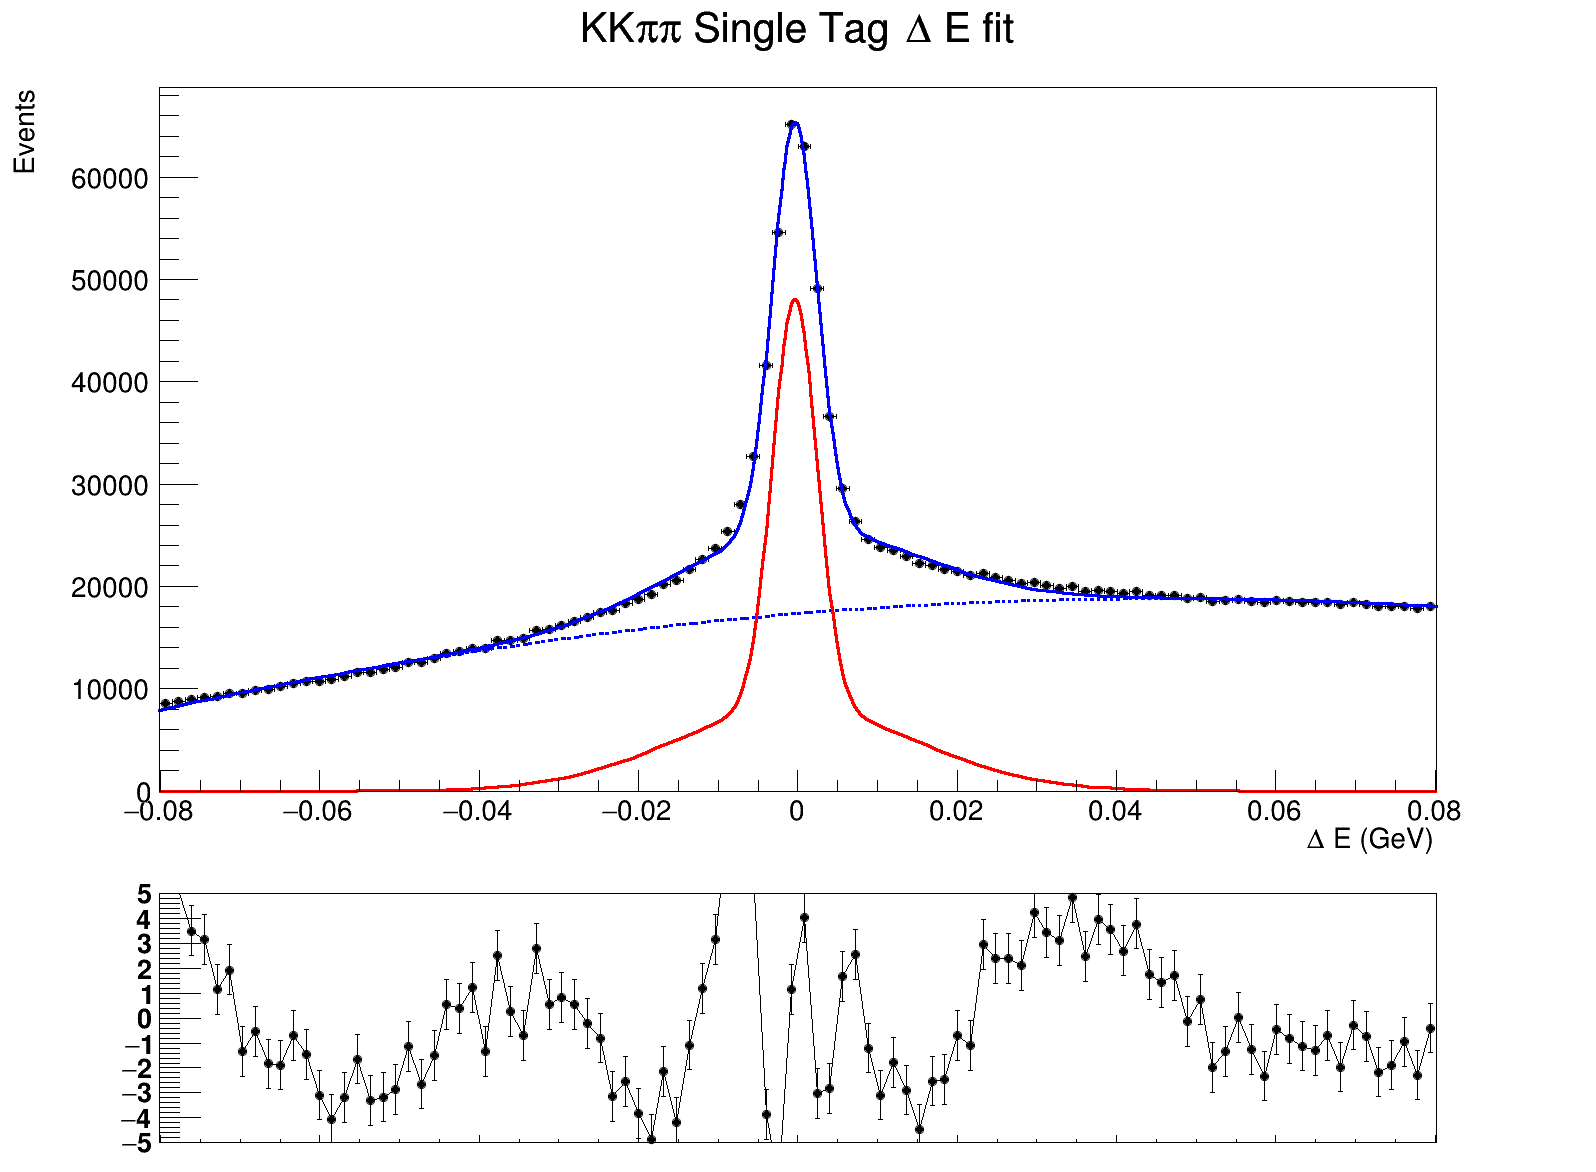
\includegraphics[width=\textwidth]{KKpipiSingleTagDeltaEPlotMCOld.png}
      \caption{$\Delta E$, MC}
    \end{subfigure}
  \end{figure}
  Problem: Why is there a broad + narrow peak?
\end{frame}

\begin{frame}{Broad peak from combinatorial background}
  \begin{figure}
    \centering
    \begin{subfigure}{0.5\textwidth}
      \centering
      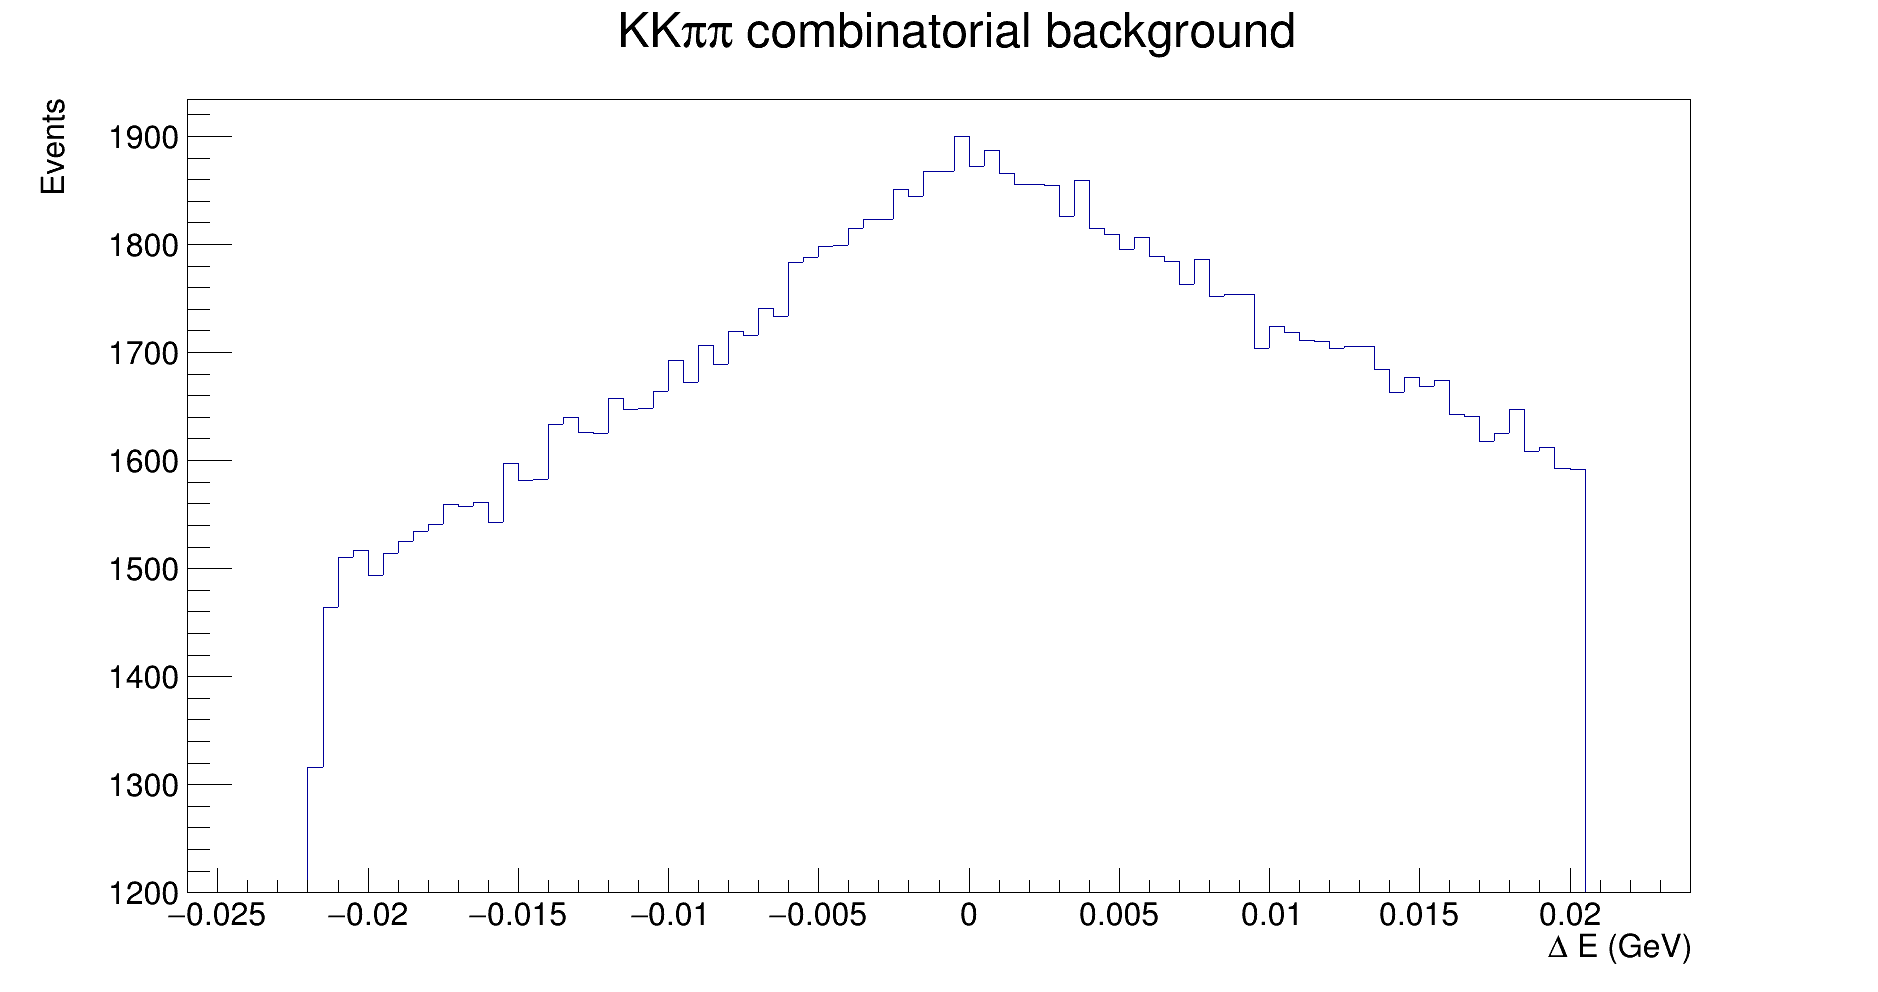
\includegraphics[width=\textwidth]{KKpipiDeltaECombinatorial.png}
      \caption{$\Delta E$, inclusive MC combinatorial background}
    \end{subfigure}%
    \begin{subfigure}{0.5\textwidth}
      \centering
      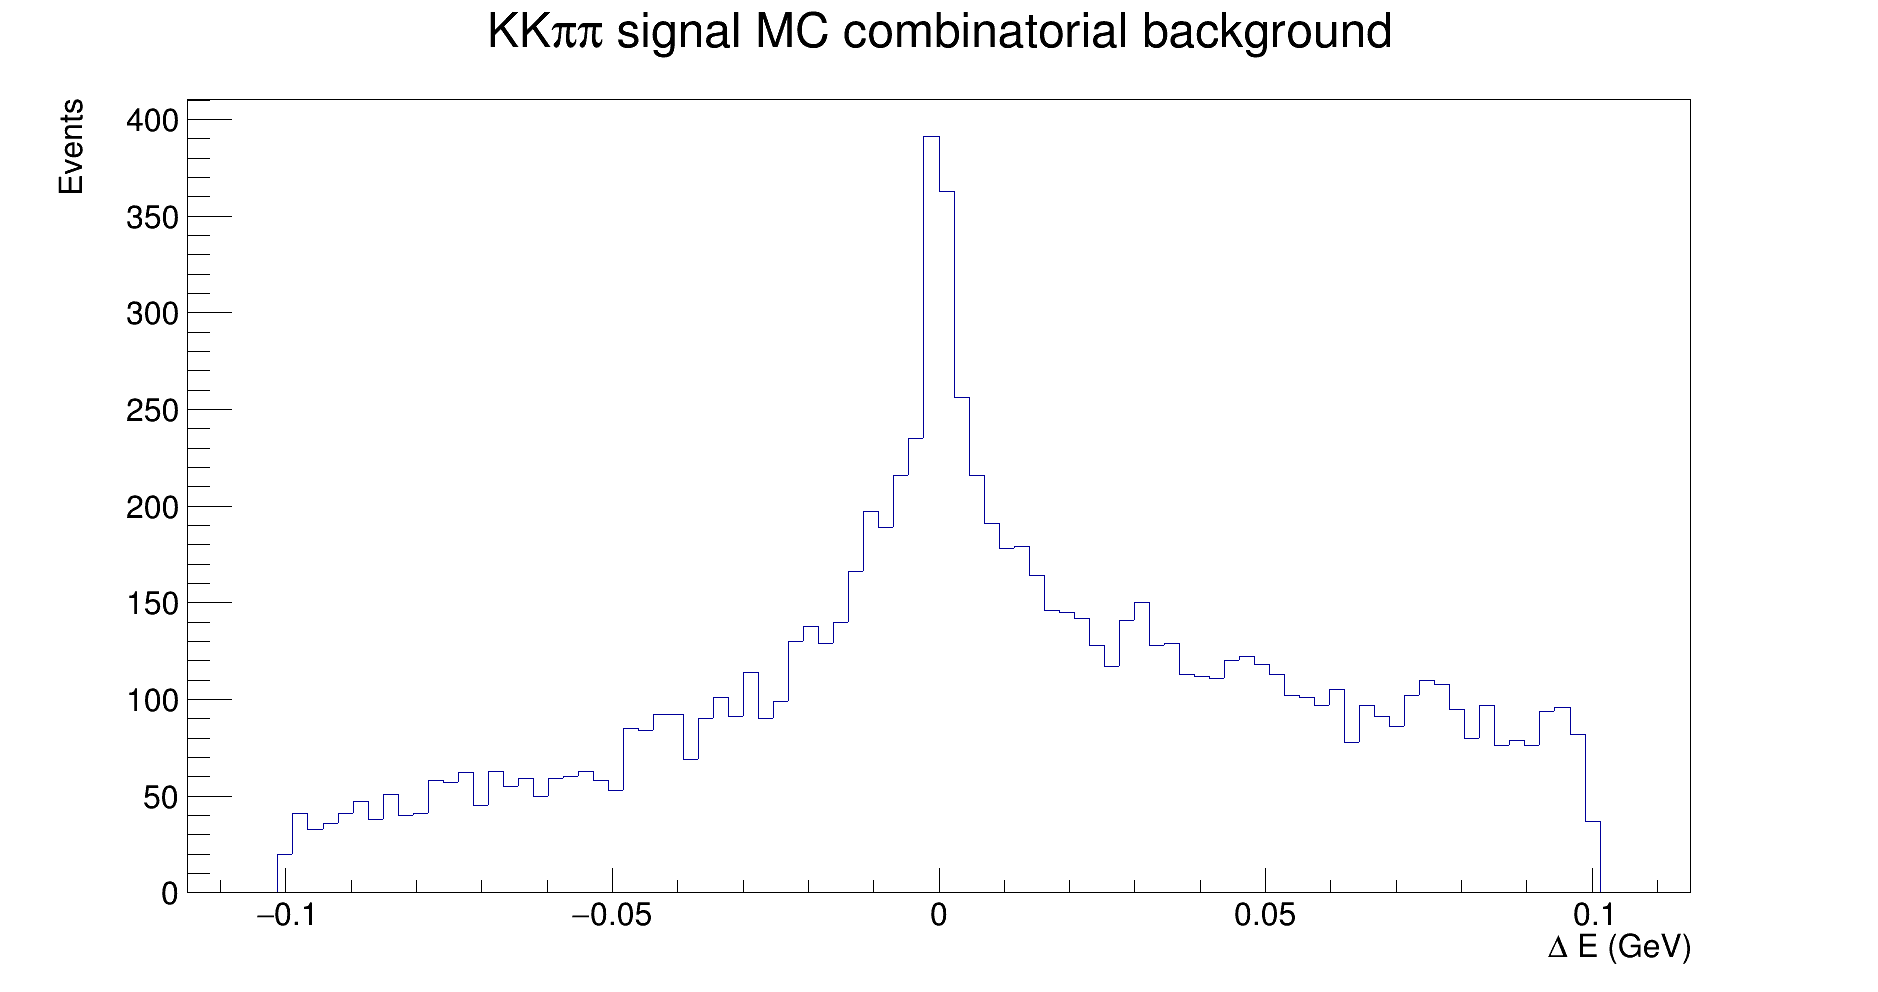
\includegraphics[width=\textwidth]{KKpipiDeltaECombinatorialSignalMC.png}
      \caption{$\Delta E$, signal MC combinatorial background}
    \end{subfigure}
  \end{figure}
  \begin{itemize}
    \item{Sharp peak/kink near $\Delta E = 0$ in combinatorial background}
    \item{No particular component that causes this}
  \end{itemize}
\end{frame}

\begin{frame}{Comparison with $K\pi\pi\pi$ combinatorial background}
  \begin{figure}
    \centering
    \begin{subfigure}{0.5\textwidth}
      \centering
      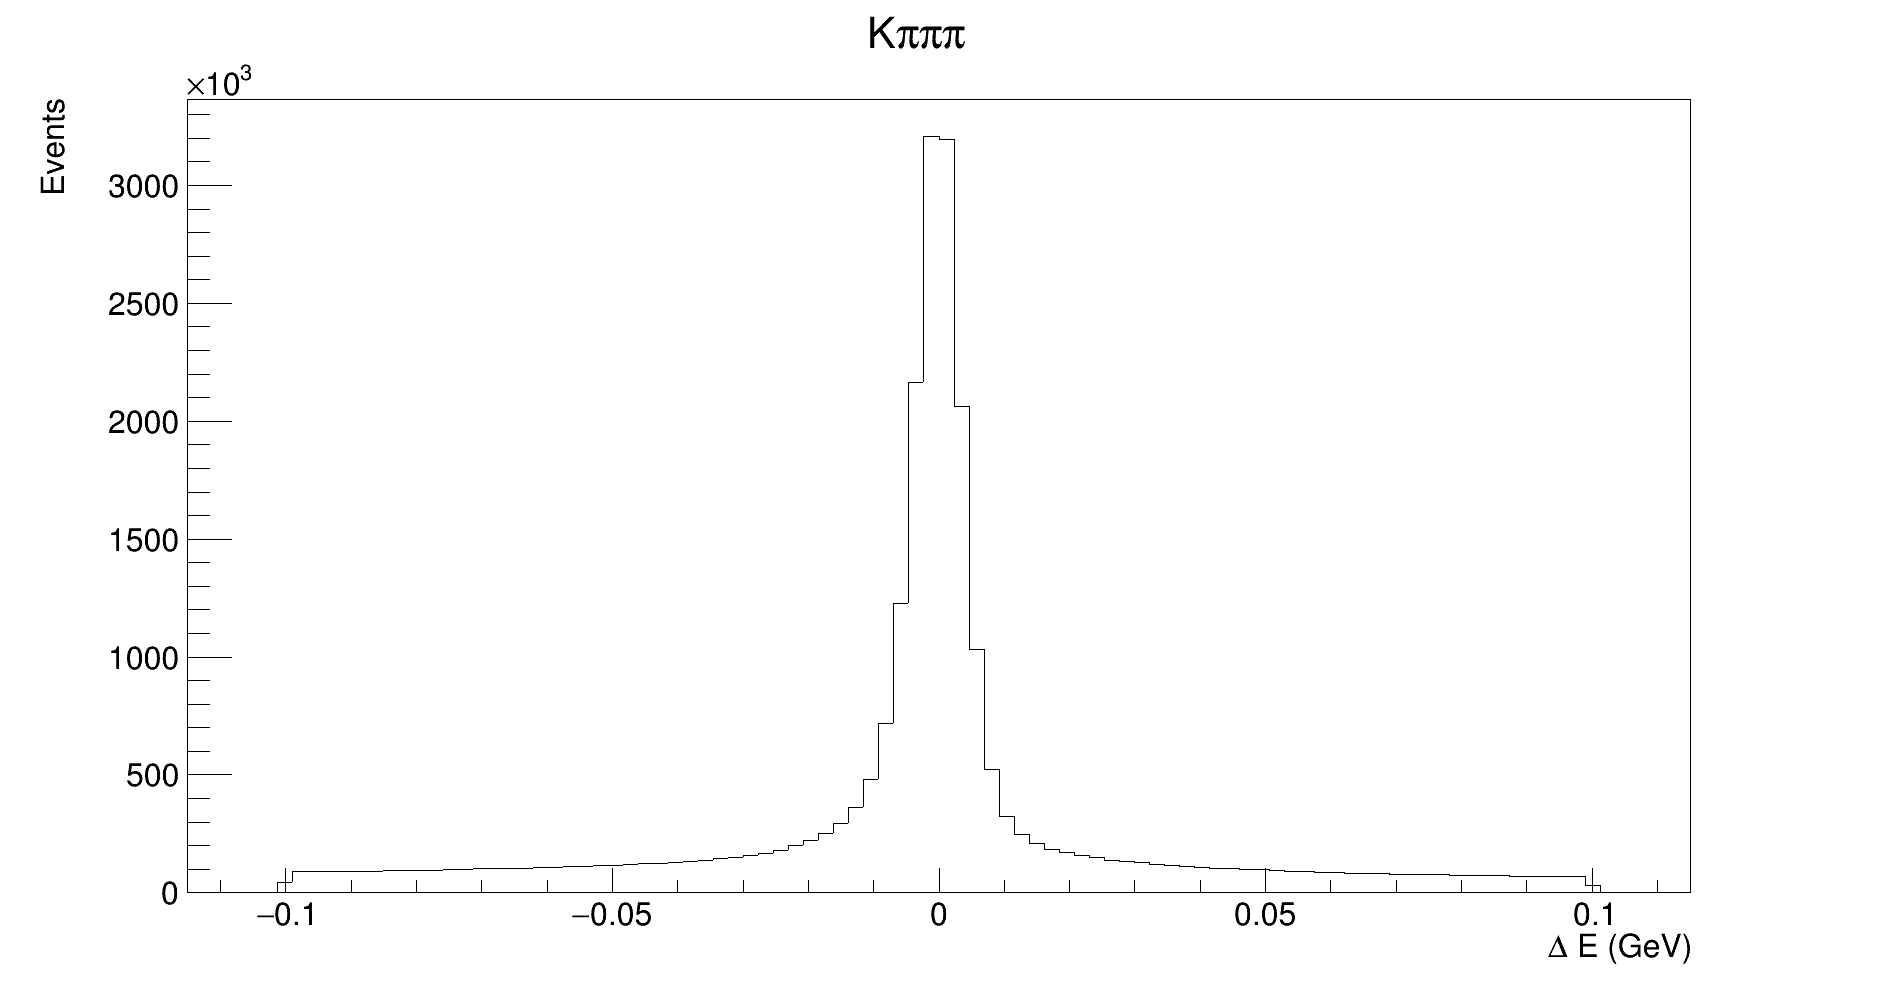
\includegraphics[width=\textwidth]{KpipipiDeltaE.png}
      \caption{$\Delta E$ from $K\pi\pi\pi$ single tag, inclusive $D^0\bar{D^0}$ MC}
    \end{subfigure}%
    \begin{subfigure}{0.5\textwidth}
      \centering
      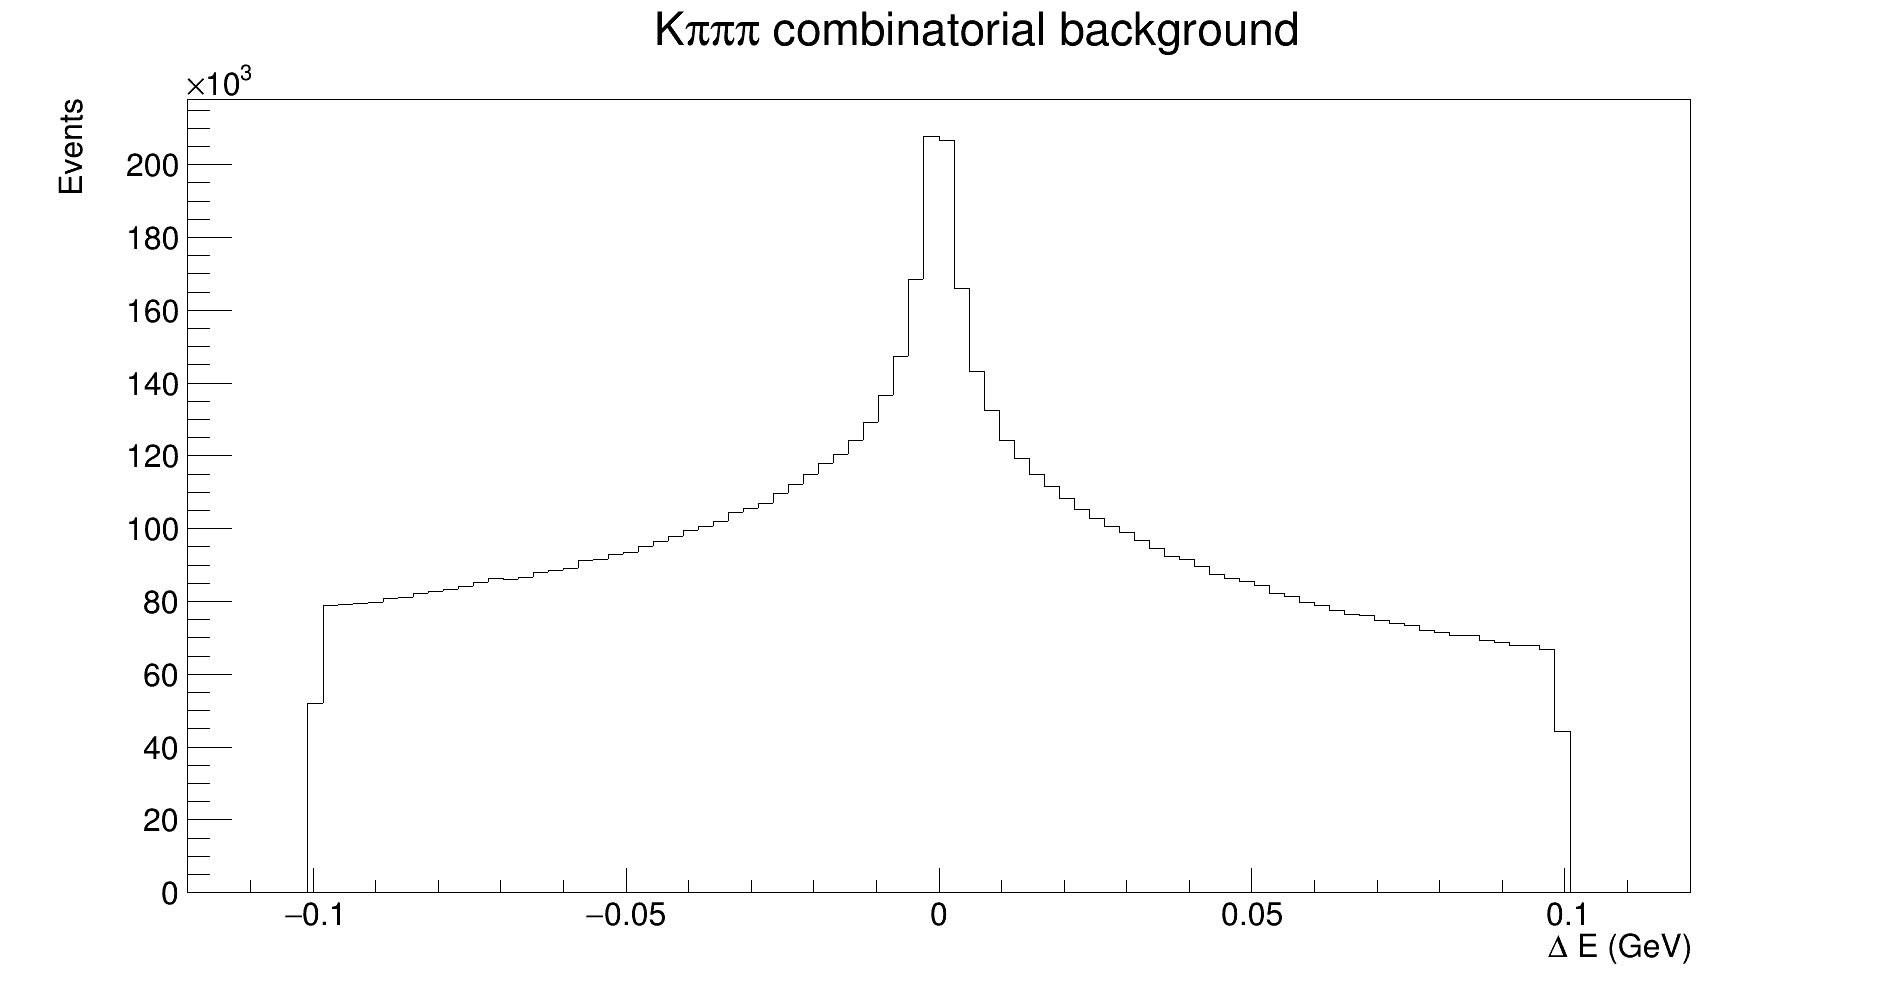
\includegraphics[width=\textwidth]{KpipipiDeltaECombinatorial.png}
      \caption{$\Delta E$ from $K\pi\pi\pi$ combinatorial background, inclusive $D^0\bar{D^0}$ MC}
    \end{subfigure}
  \end{figure}
  \begin{itemize}
    \item{See a similar sharp peak/kink for $K\pi\pi\pi$}
    \item{Not noticeble under the large signal}
  \end{itemize}
\end{frame}

\begin{frame}{Possible explanation for $\Delta E$ shape}
  \begin{itemize}
    \setlength\itemsep{2em}
    \item{Had a closer look at all single tag $\Delta E$ distributions:}
    \begin{itemize}
      \item{Larger peak in modes with high track multiplicity}
      \item{See a similar, but smaller peak in all 3-body modes}
      \item{No peak for 2-body modes}
    \end{itemize}
    \item{Bias in $\Delta E$ because of selection:}
    \begin{itemize}
      \item{DTagTool: For events with multiple candidates, pick candidates with smallest $\Delta E$}
      \item{For events with many track combinations, this will favour background near $\Delta E = 0$.}
    \end{itemize}
  \end{itemize}
\end{frame}

\begin{frame}{Thought experiment to explain the peak}
  \begin{itemize}
    \item{Consider a uniform combinatorial background in $\Delta E$}
    \item{Generate $N$ random numbers between $-0.1$ and $0.1$}
    \item{Pick number closest to $\Delta E = 0$}
    \item{Resulting $\Delta E$ distribution has a peak/kink at $\Delta E = 0$}
  \end{itemize}
  \begin{figure}
    \centering
    \begin{subfigure}{0.33\textwidth}
      \centering
      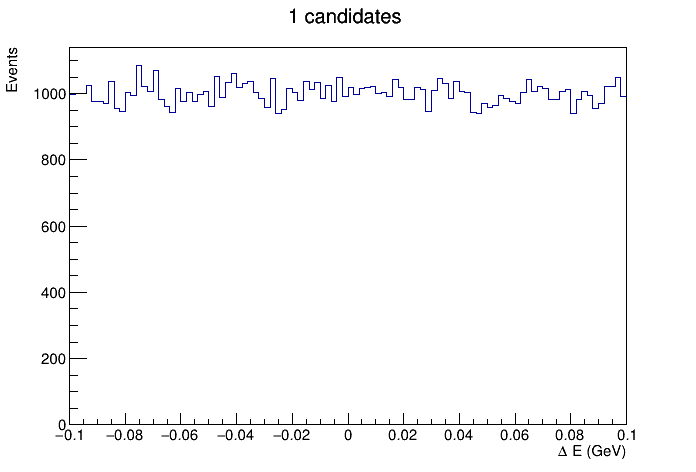
\includegraphics[width=\textwidth]{DeltaEPeaking1.png}
    \end{subfigure}%
    \begin{subfigure}{0.33\textwidth}
      \centering
      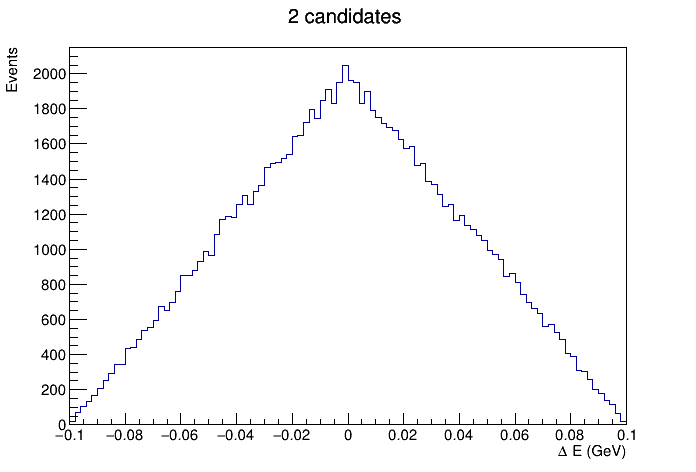
\includegraphics[width=\textwidth]{DeltaEPeaking2.png}
    \end{subfigure}%
    \begin{subfigure}{0.33\textwidth}
      \centering
      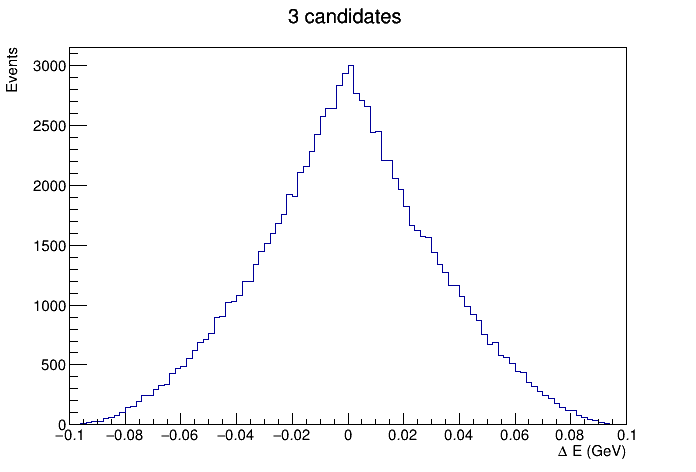
\includegraphics[width=\textwidth]{DeltaEPeaking3.png}
    \end{subfigure}
  \end{figure}
\end{frame}

\begin{frame}{How to deal with this?}
  \begin{itemize}
    \setlength\itemsep{2em}
    \item{Peak at $\Delta E$ seems to be caused by the selection itself, can't remove with cuts}
    \item{Instead, modify PDF shape}
    \begin{itemize}
      \item{Before: $f(x) = 1 + ax + bx^2$}
      \item{Change to: Two independent polynomials on either side}
      \begin{itemize}
        \item{$f(x) = 1 + a_1x + b_1x^2, \quad \Delta E < 0$}
        \item{$f(x) = 1 + a_2x + b_2x^2, \quad \Delta E > 0$}
      \end{itemize}
    \end{itemize}
  \end{itemize}
\end{frame}

\begin{frame}{New $\Delta E$ fit in data vs MC}
  \begin{figure}
    \centering
    \begin{subfigure}{0.5\textwidth}
      \centering
      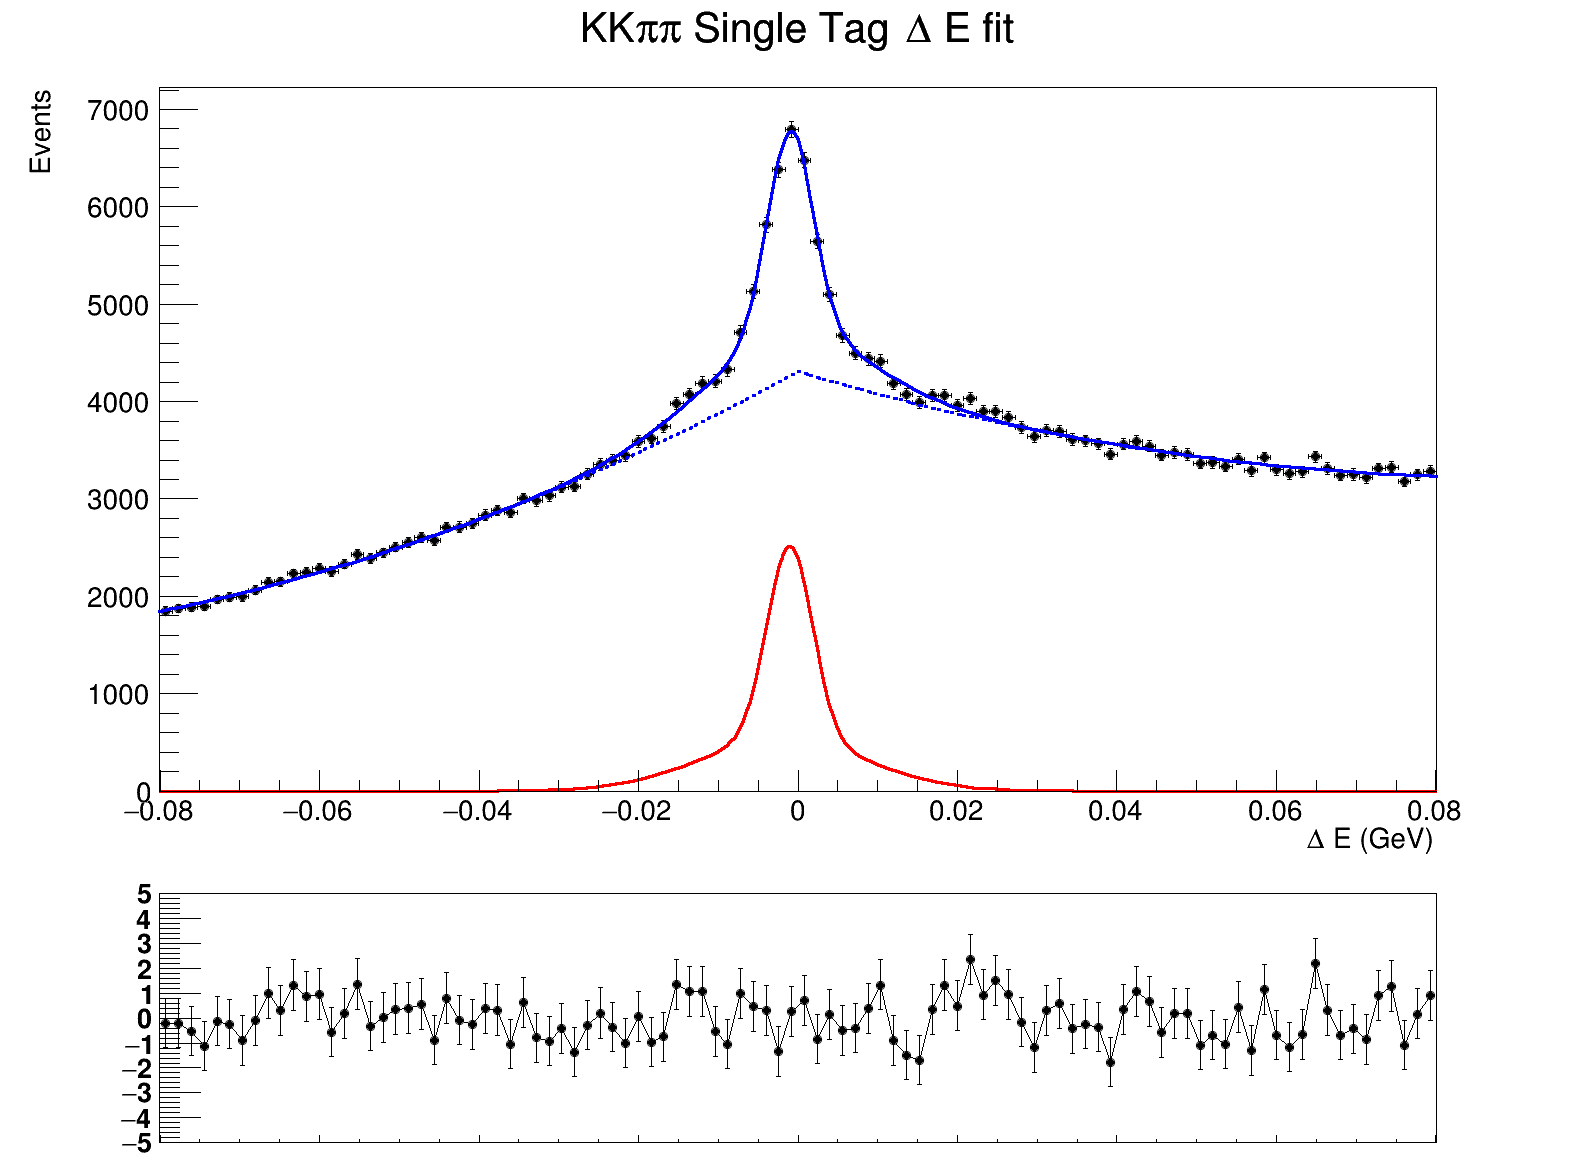
\includegraphics[width=\textwidth]{KKpipiDeltaEPlotData.png}
      \caption{$\Delta E$, data}
    \end{subfigure}%
    \begin{subfigure}{0.5\textwidth}
      \centering
      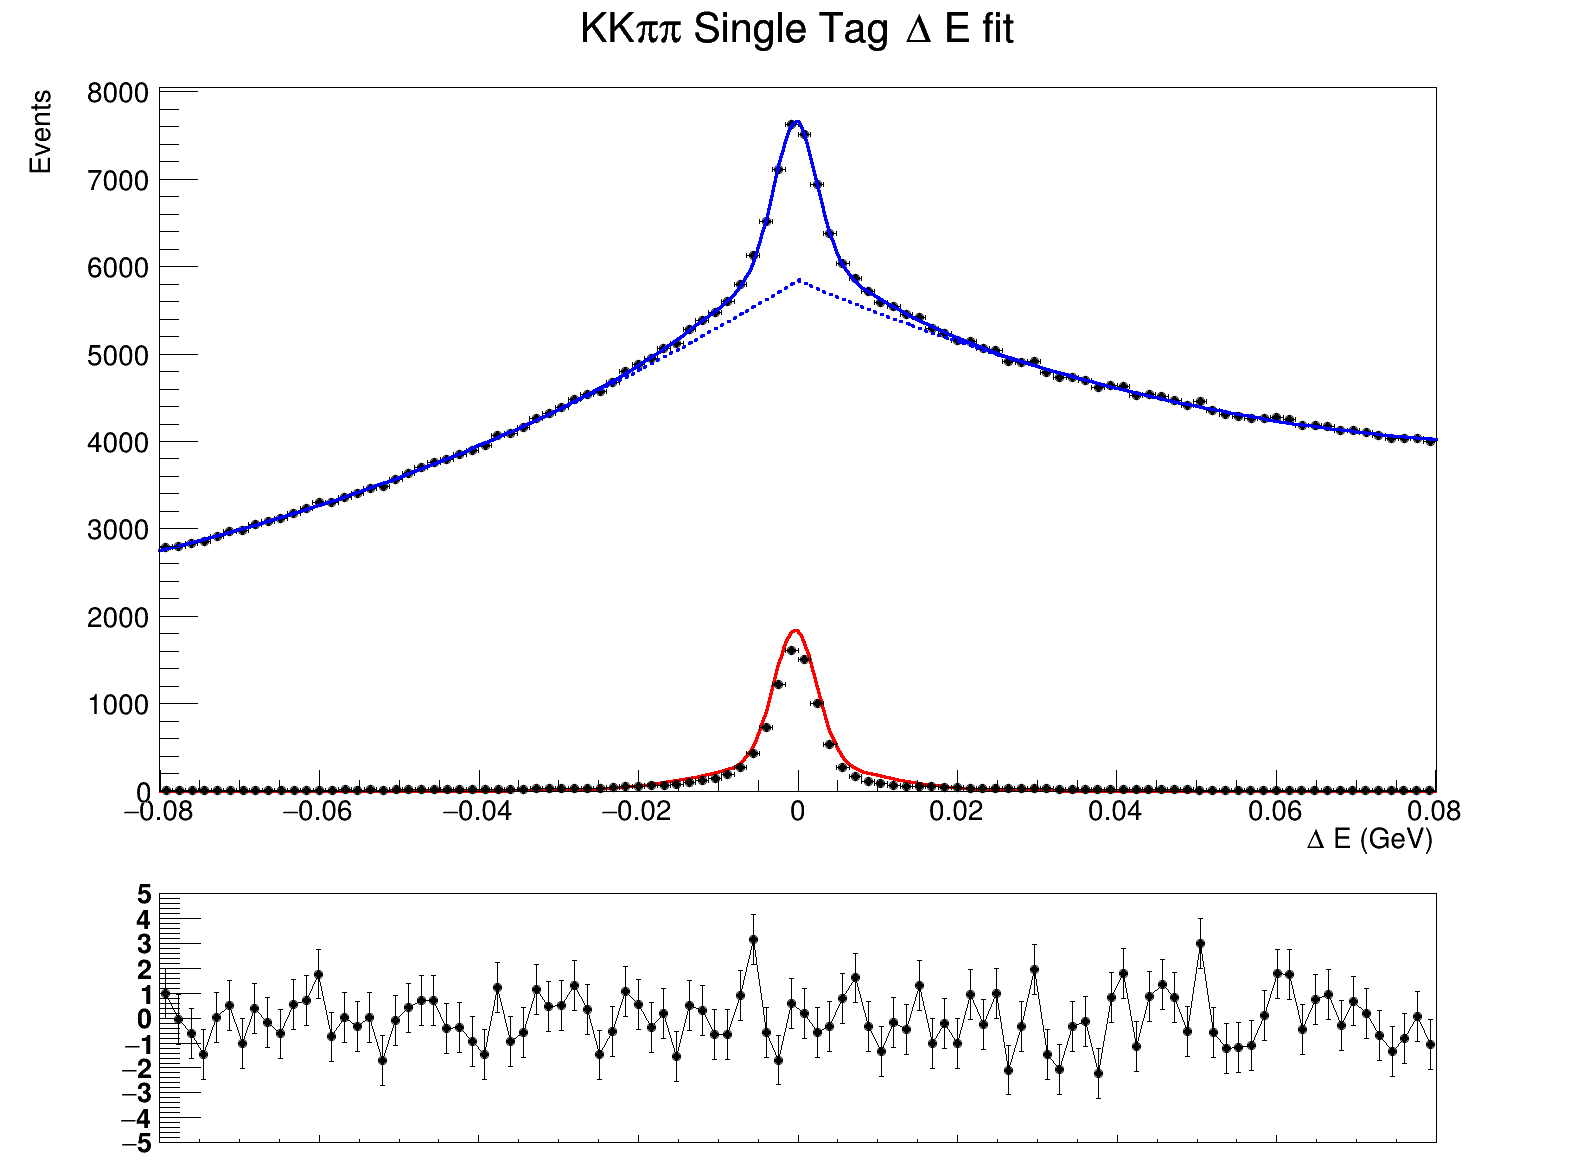
\includegraphics[width=\textwidth]{KKpipiDeltaEPlotMC.png}
      \caption{$\Delta E$, MC}
    \end{subfigure}
  \end{figure}
\end{frame}

\begin{frame}{Previous $\Delta E$ fit in data vs MC}
  \begin{figure}
    \centering
    \begin{subfigure}{0.5\textwidth}
      \centering
      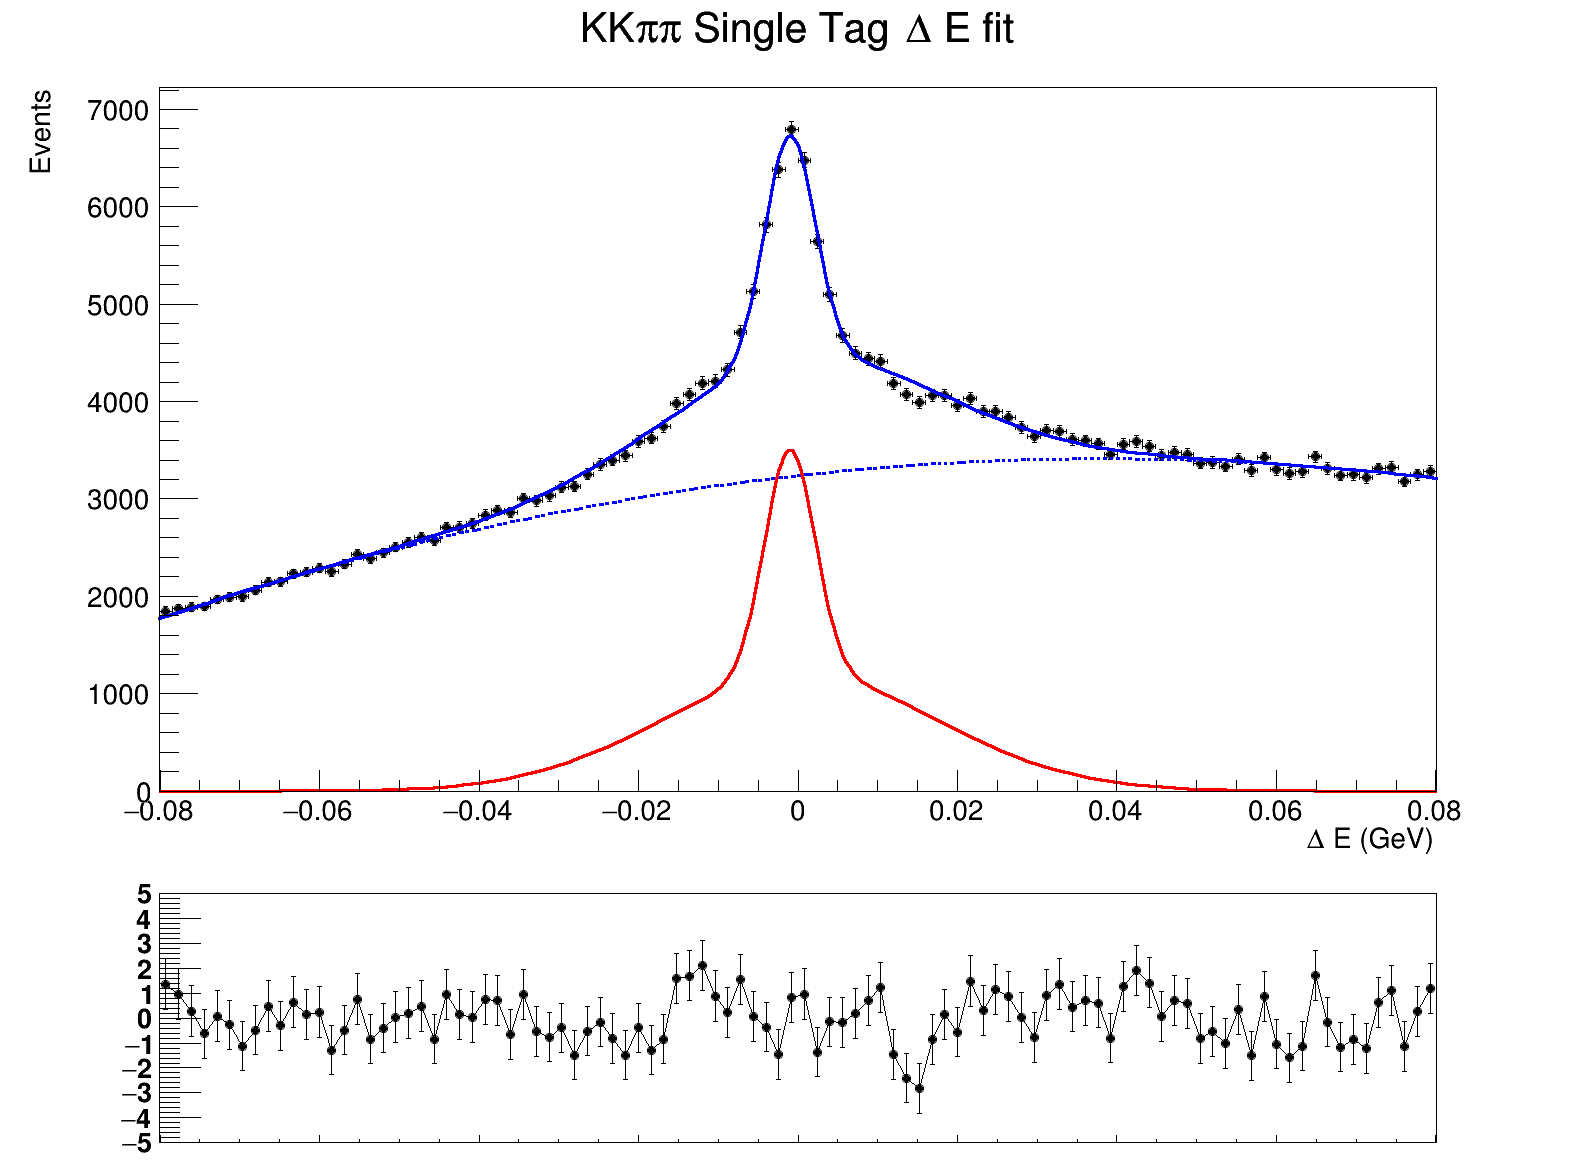
\includegraphics[width=\textwidth]{KKpipiSingleTagDeltaEPlotDataOld.png}
      \caption{$\Delta E$, data}
    \end{subfigure}%
    \begin{subfigure}{0.5\textwidth}
      \centering
      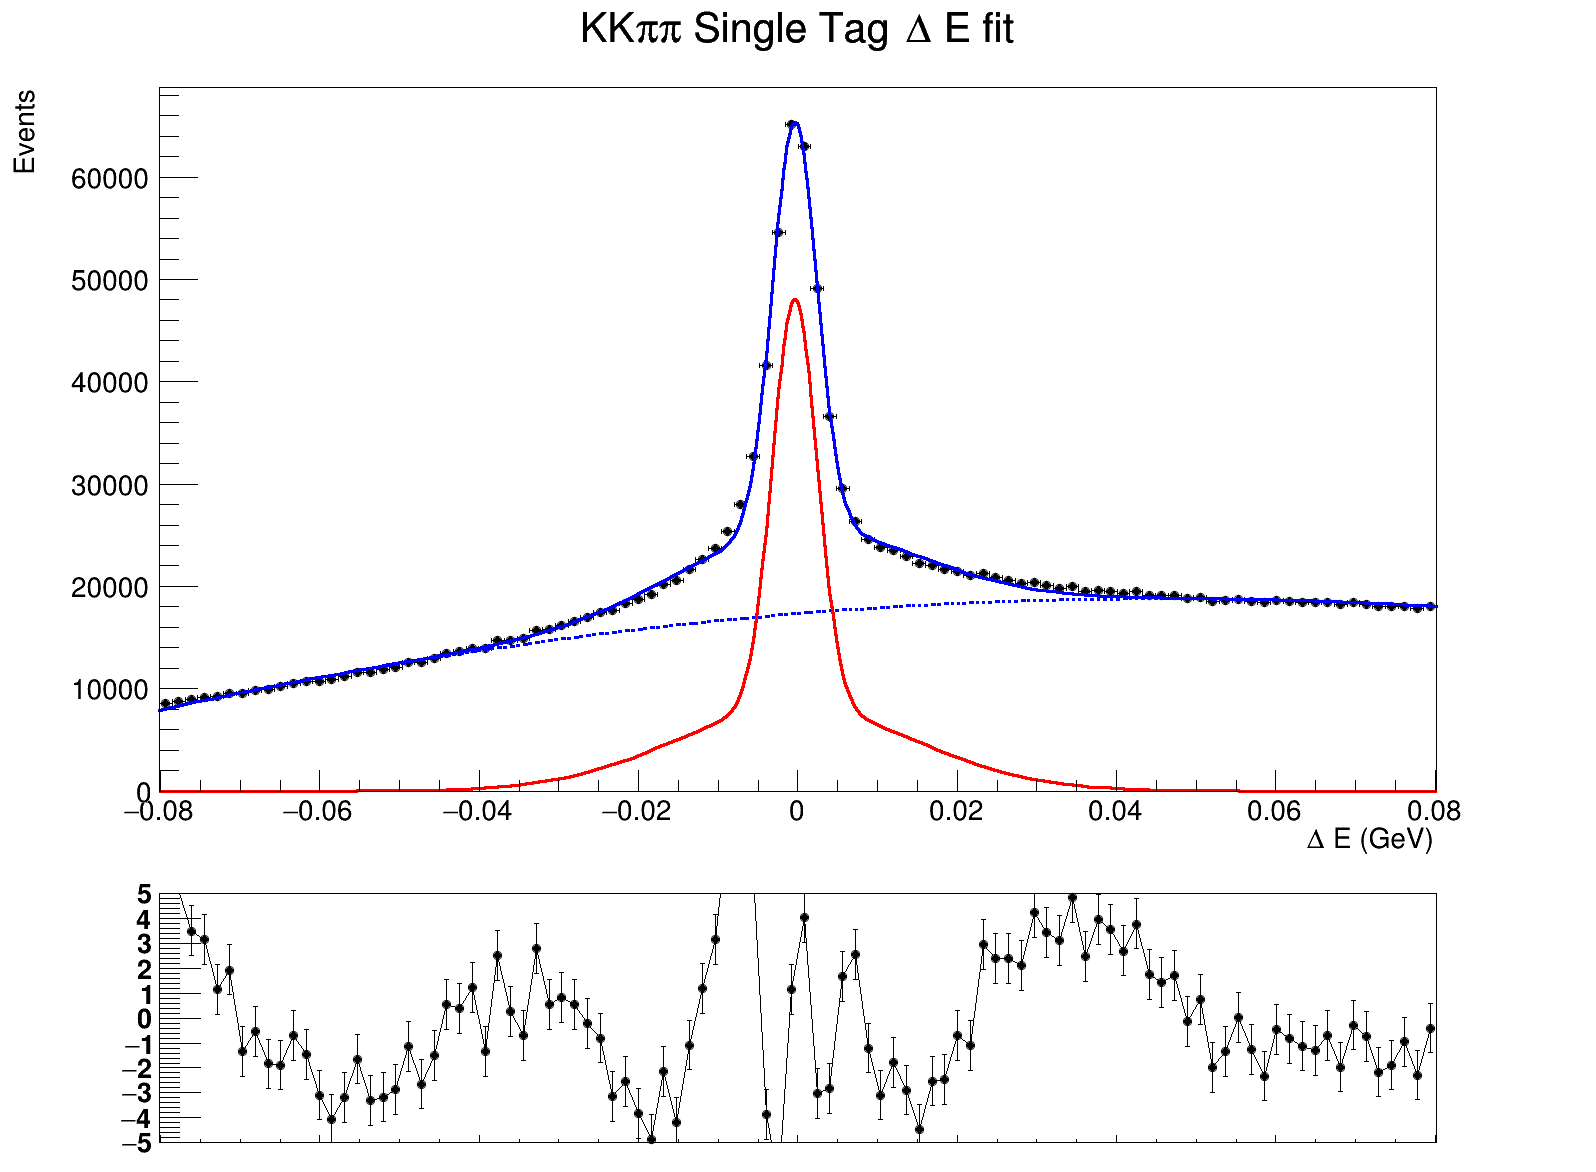
\includegraphics[width=\textwidth]{KKpipiSingleTagDeltaEPlotMCOld.png}
      \caption{$\Delta E$, MC}
    \end{subfigure}
  \end{figure}
\end{frame}

\section{$K_SKK$ peaking background}
\begin{frame}{$K_SKK$ peaking background}
  \begin{itemize}
    \setlength\itemsep{2em}
    \item{Generated a signal MC sample of $K_SKK$, reconstructed as $KK\pi\pi$}
    \item{Applied flight significance cut at $2$}
    \item{Out of $200000$ generated events, $6883$ events made it through this selection ($3\%$)}
  \end{itemize}
\end{frame}

\begin{frame}{$K_SKK$ peaking background}
  \begin{figure}
    \centering
    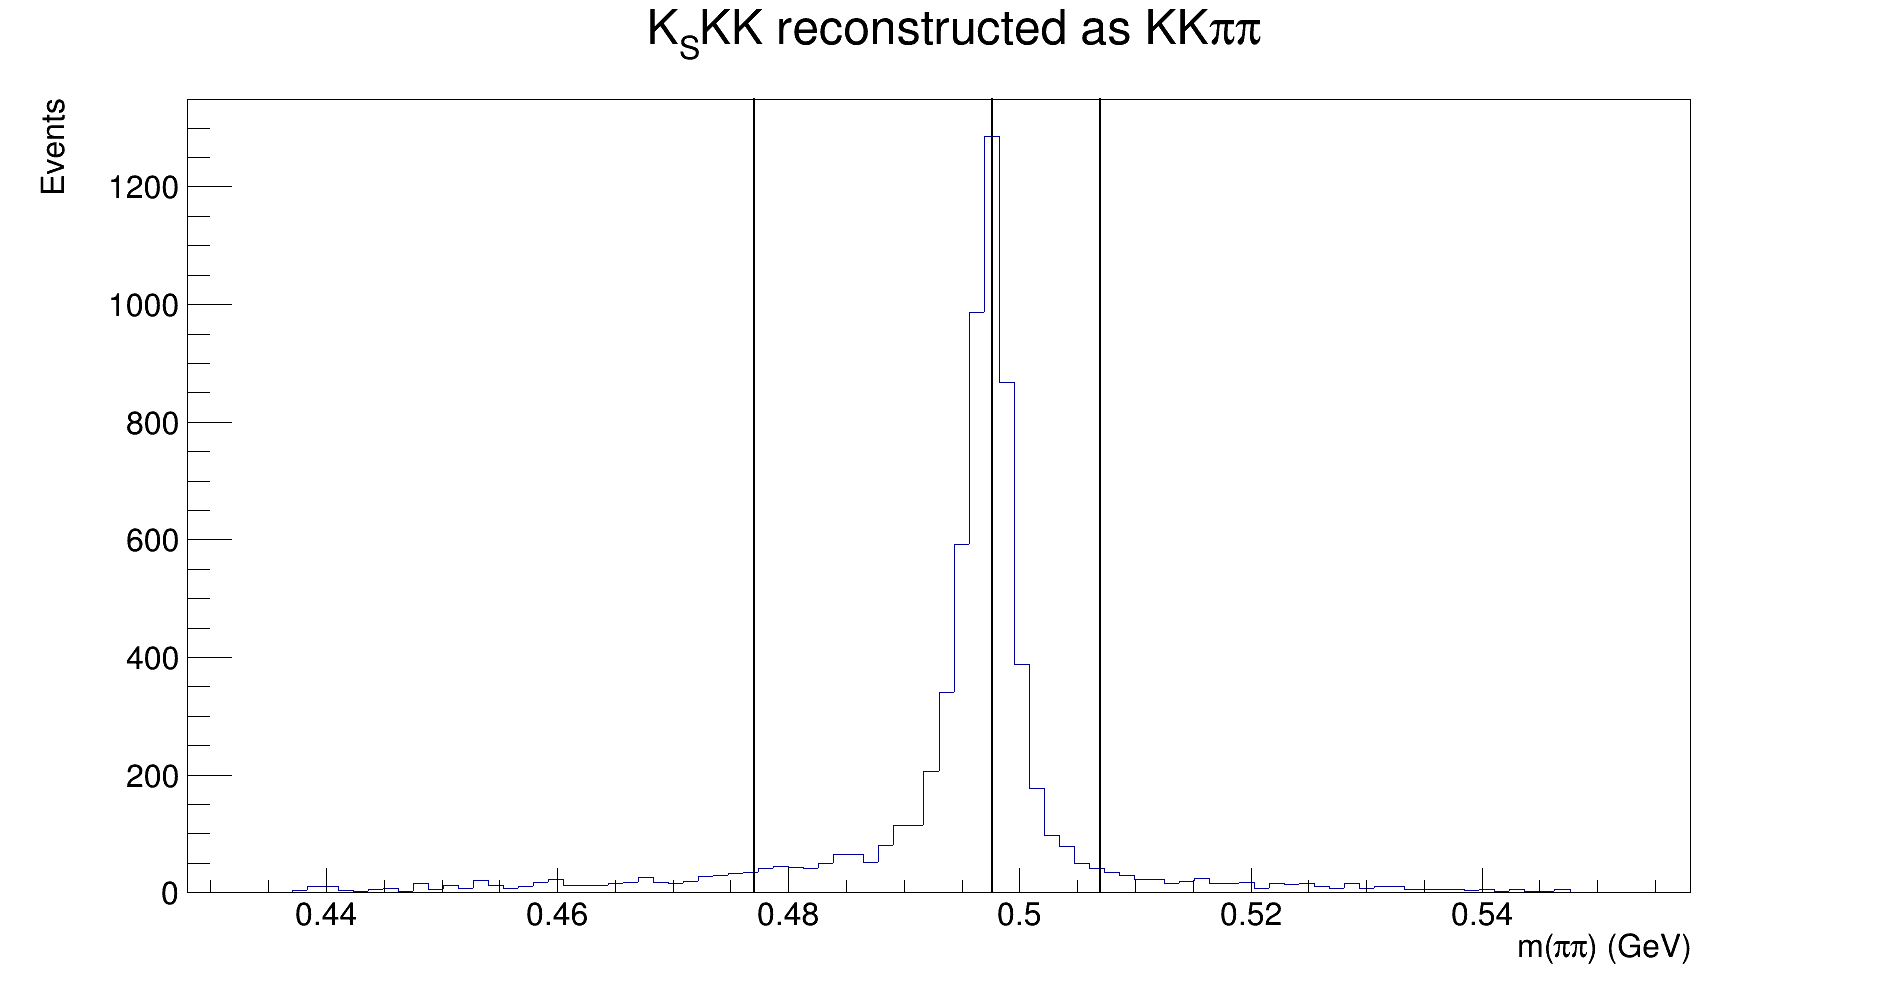
\includegraphics[width=0.8\textwidth]{MpipiVeto.png}
    \caption{$\pi\pi$ invariant mass in $K_SKK$ peaking background}
  \end{figure}
  \begin{itemize}
    \item{A veto at $\SI{477}{\mega\eV} < m(\pi\pi) < \SI{507}{\mega\eV}$ removes $85\%$ of the remaining background}
  \end{itemize}
\end{frame}

\section{$KK\pi\pi$ single tag components}
\begin{frame}{$KK\pi\pi$ single tag components}
  \begin{figure}
    \centering
    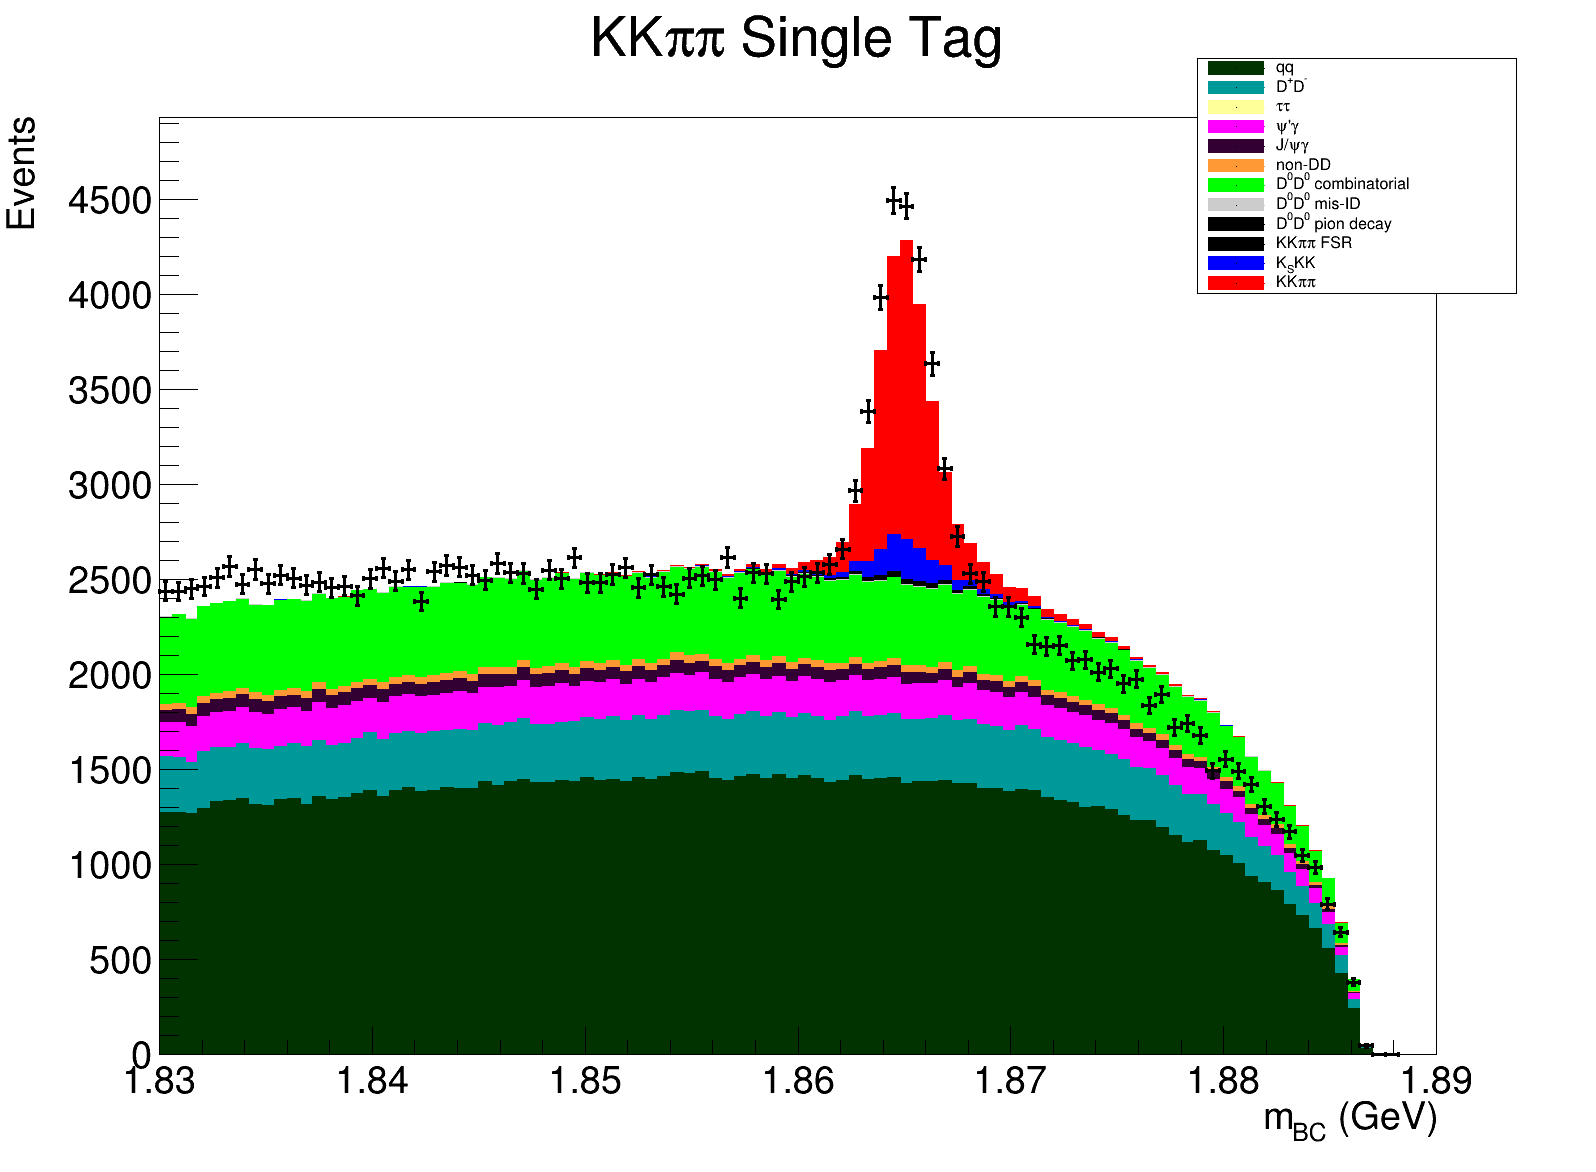
\includegraphics[width=0.8\textwidth]{MCPlusDataOld.png}
    \caption{$KK\pi\pi$ single tag $m_\text{BC}$ components}
  \end{figure}
\end{frame}

\begin{frame}{$KK\pi\pi$ single tag components}
  \begin{figure}
    \centering
    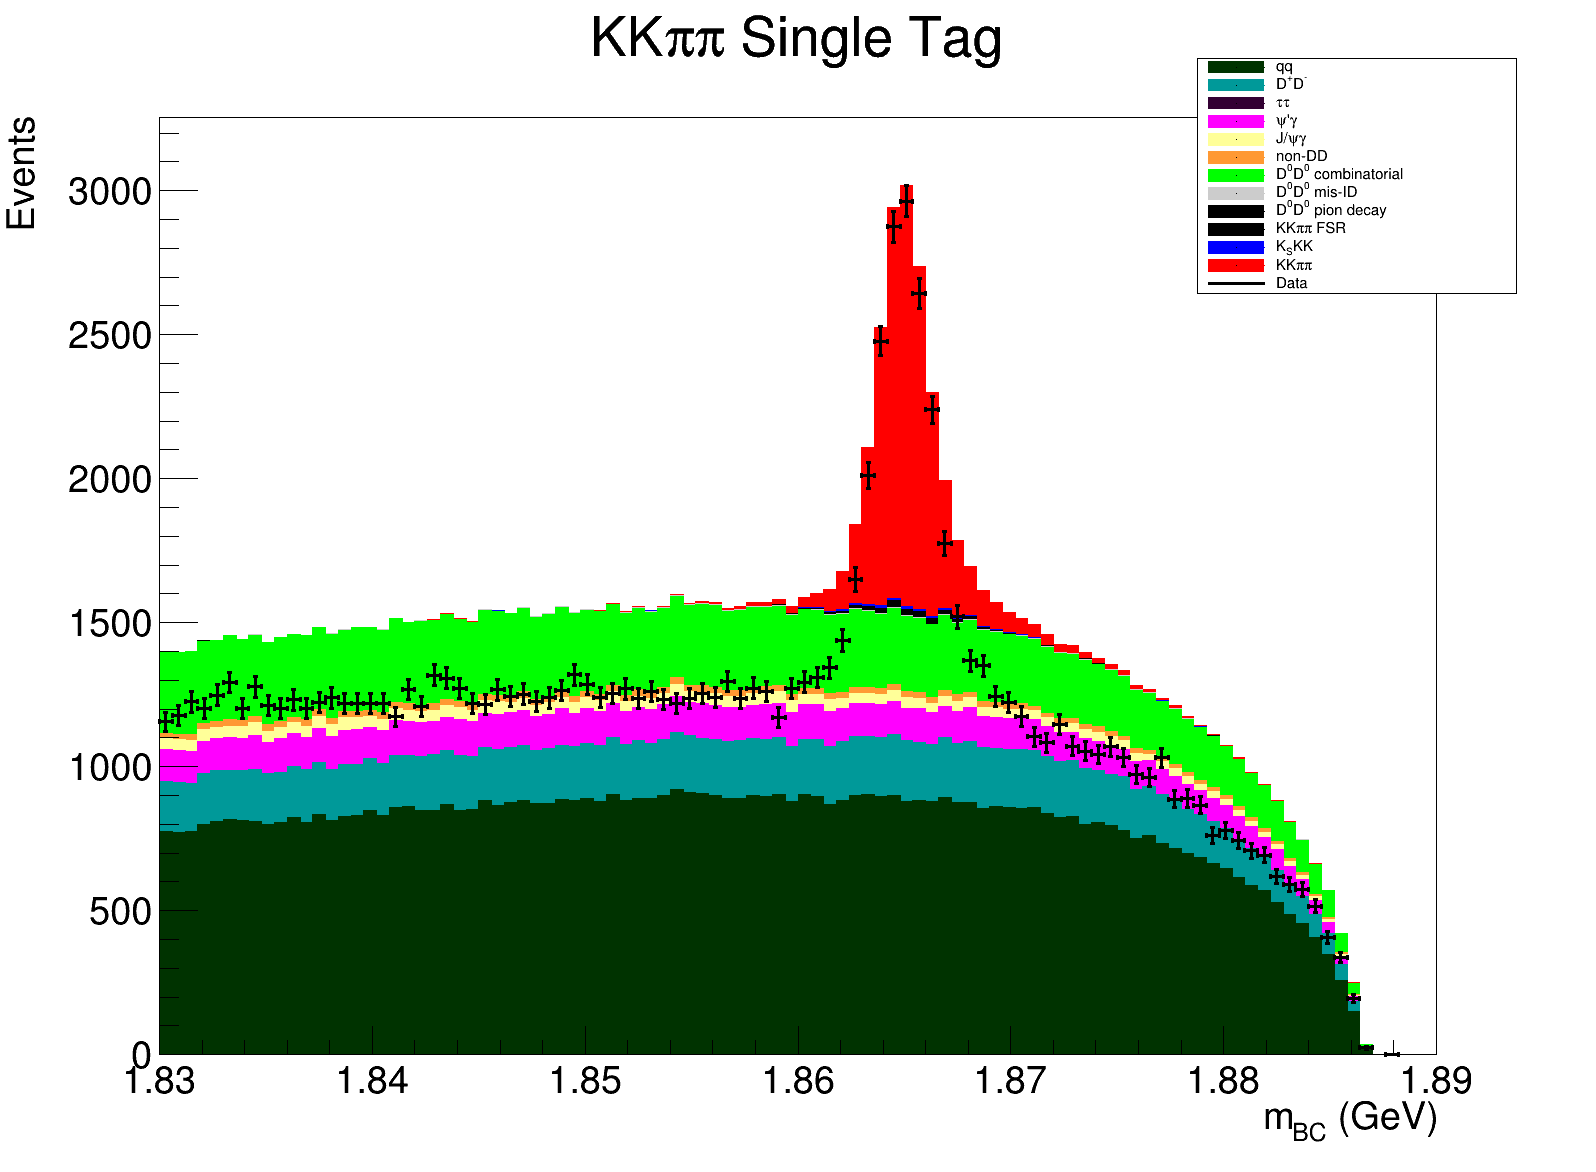
\includegraphics[width=0.8\textwidth]{MCPlusData.png}
    \caption{$KK\pi\pi$ single tag $m_\text{BC}$ components}
  \end{figure}
\end{frame}

\begin{frame}{$KK\pi\pi$ single tag components}
  \begin{figure}
    \centering
    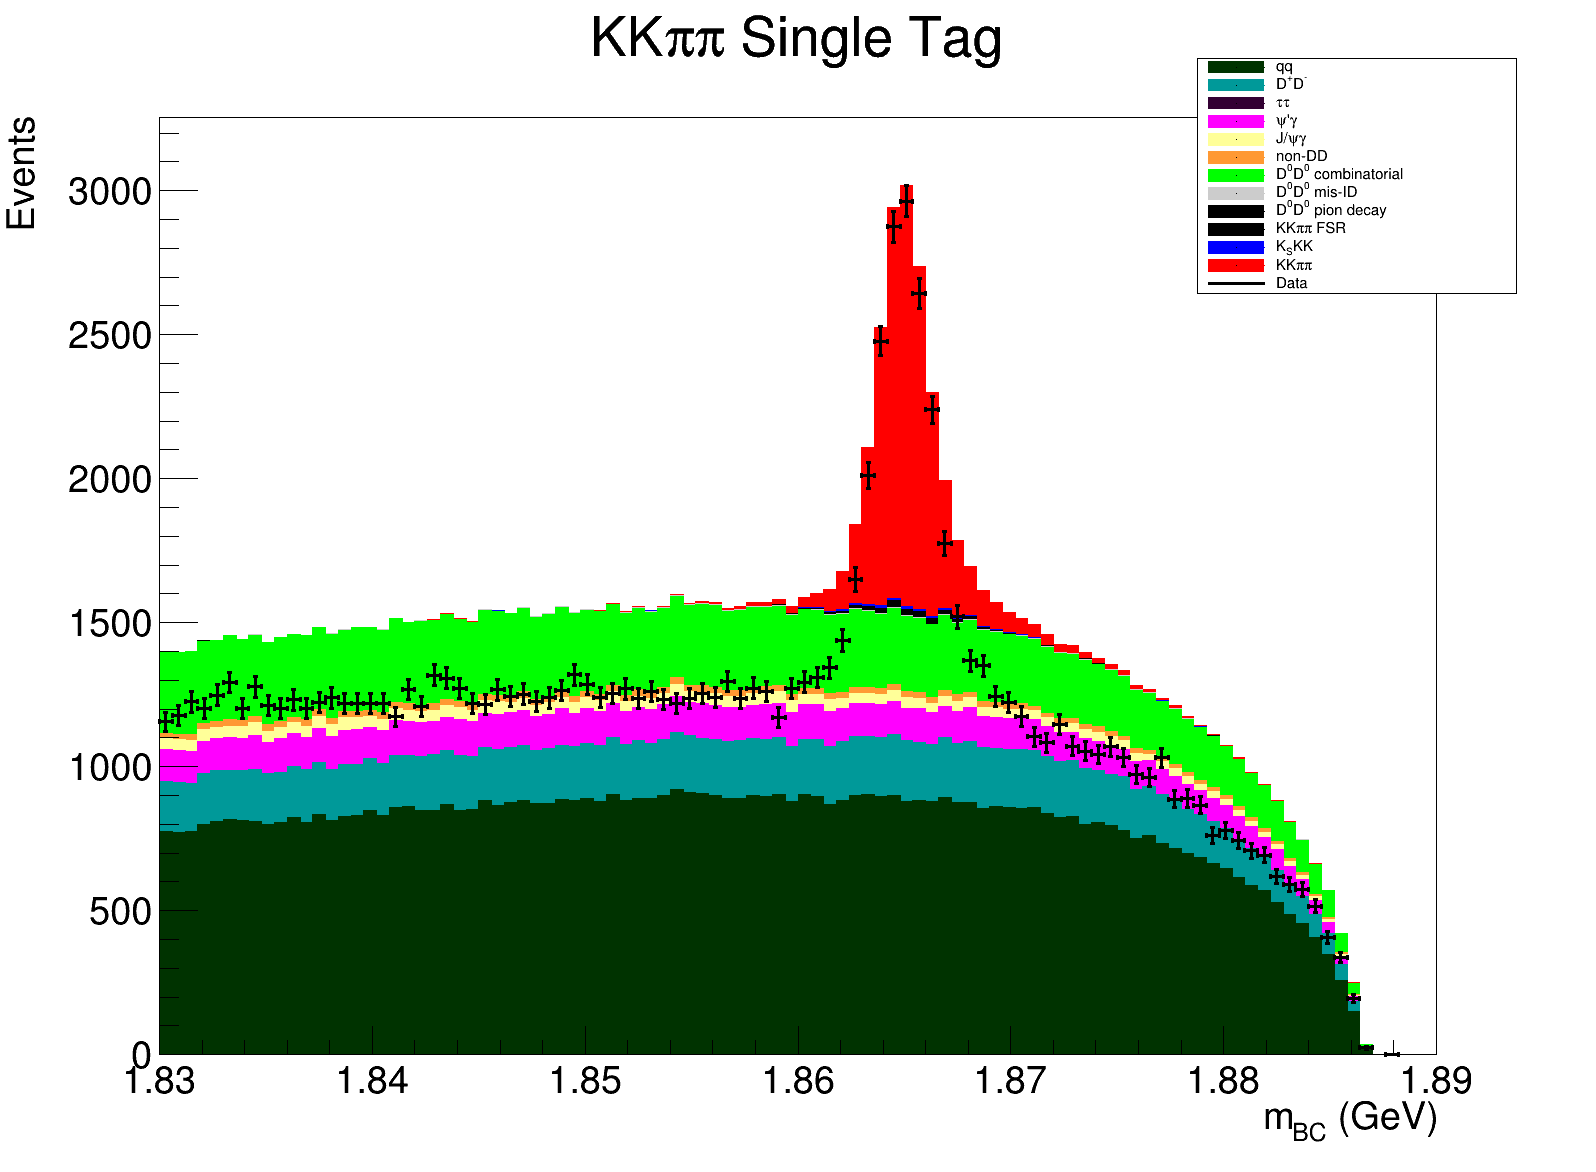
\includegraphics[width=0.4\textwidth]{MCPlusData.png}
    \caption{$KK\pi\pi$ single tag $m_\text{BC}$ components}
  \end{figure}
  \begin{itemize}
    \item{$K_SKK$ background is very small}
    \item{Combinatorial background lower in data}
    \item{Signal larger in data, possibly because branching fraction is lower in decay card ($15\%$)}
  \end{itemize}
\end{frame}

\section{Next steps}
\begin{frame}{Next steps}
  \begin{itemize}
    \setlength\itemsep{2em}
    \item{Run same studies on other modes}
    \item{Start with DT yields, check with expectation from amplitude model}
  \end{itemize}
\end{frame}

\end{document}
